\addcontentsline{toc}{chapter}{Appendix 10}\label{ch:SimJitter}
\chapter{Simulator Jitter}

\section{Context}
During the testing of the NAMURU reciever, issues with the performance were identified. During thesting, the reciever was failing to sustain pahselock, resulting in an inability to track the signal. By conducting a thorough investigation using the KeaDebug feature, the source of the excessive phase error was uncovered, and the problem was rectified. 

\section{Investigation}

Upone examining the signal generated by the simulator, a discrete, quantized pattern became evident in the frequency output. This pattern, an example of which can be seen in \ref{fig:Stepping} resulted in excessive acceleration and jerk on a periodic basis, as opposed to constant acceleration, with zero jerk. Given the type 3 tracking loops in the reciever are sensitive to jerk, the root cause of the excessive phase error had been identified. By refering to the associated manuals for the GNSS simulators owned by the school, WRITE MORE STUFF HHERE 

\begin{figure}[!htb] 
    \centering
    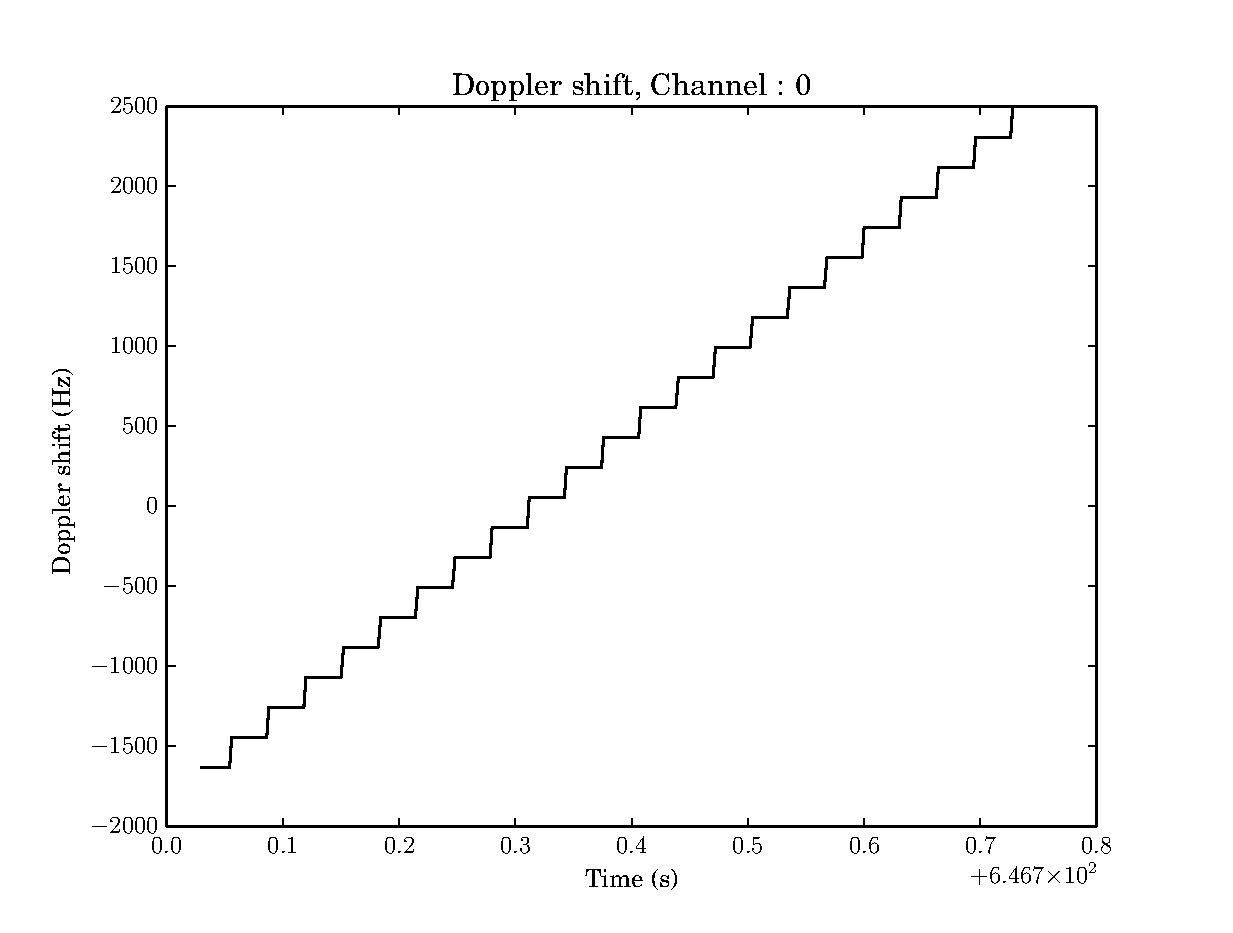
\includegraphics[width=1\textwidth]{SimulatorJitter/Stepping.eps} 
    \caption{The stepping patern observed in the frequency output of the reciever.}
    \label{fig:Stepping}
\end{figure}

\begin{figure}[!htb] 
    \centering
    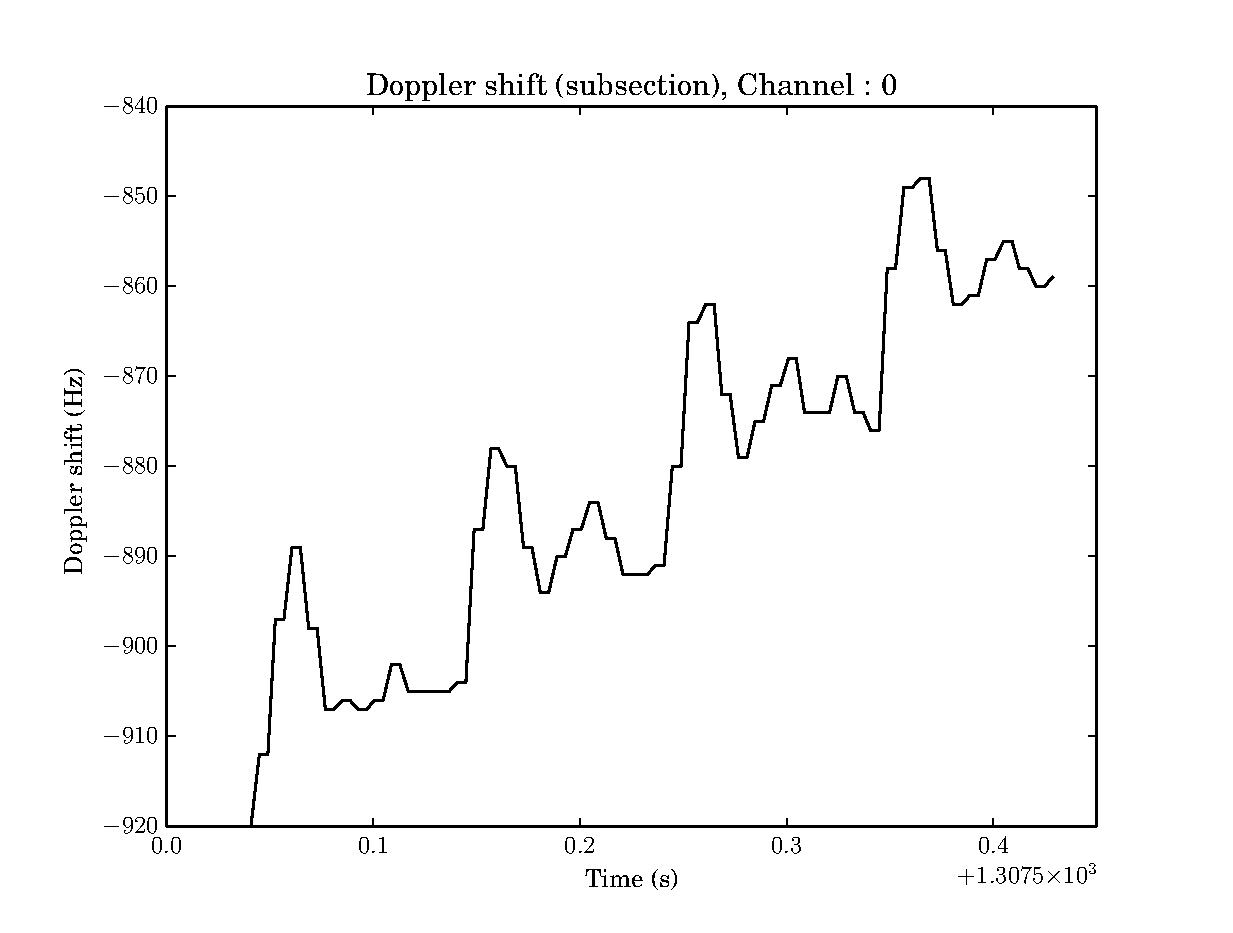
\includegraphics[width=1\textwidth]{SimulatorJitter/DopplerShiftSubsection0.eps} 
    \caption{The output from the receiver tracking looops. Notice the transient response to the step input in frequency. }
    \label{fig:}
\end{figure}

\begin{figure}[!htb] 
    \centering
    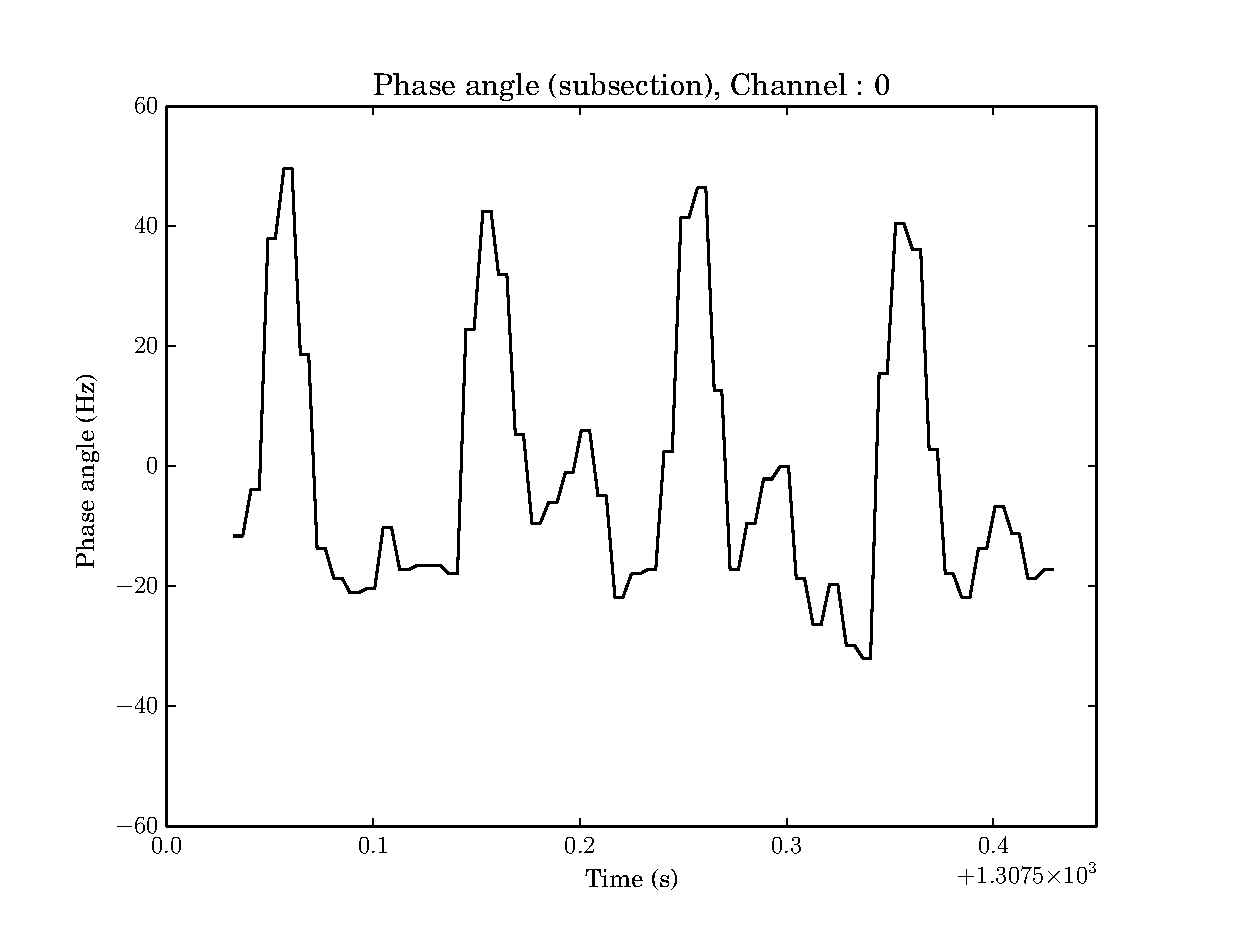
\includegraphics[width=1\textwidth]{SimulatorJitter/PhaseAngleSubsection0.eps} 
    \caption{This }
    \label{fig:}
\end{figure}

\begin{figure}[!htb] 
    \centering
    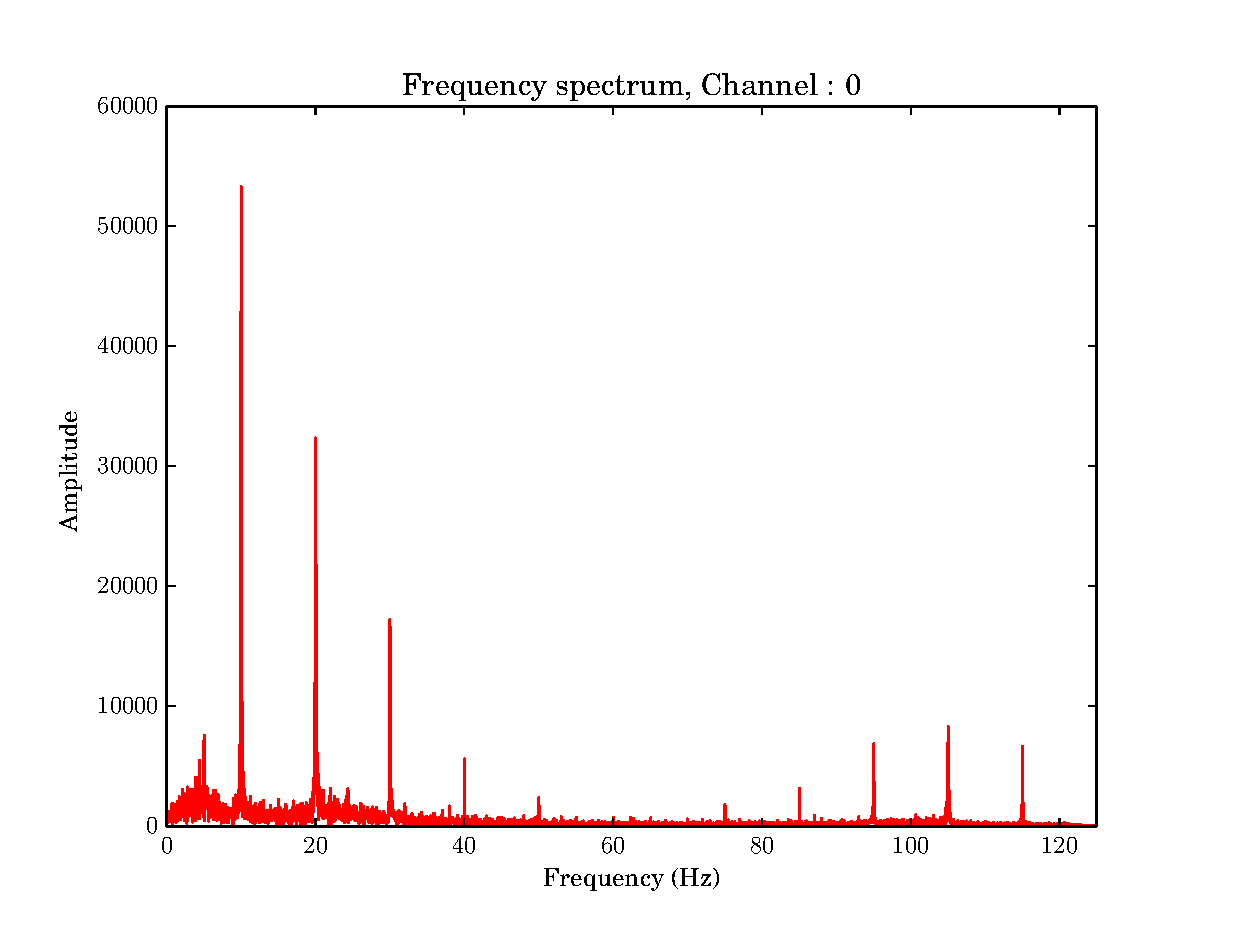
\includegraphics[width=1\textwidth]{SimulatorJitter/FFT0.eps} 
    \caption{}
    \label{fig:}
\end{figure}


\begin{figure}[!htb] 
    \centering
    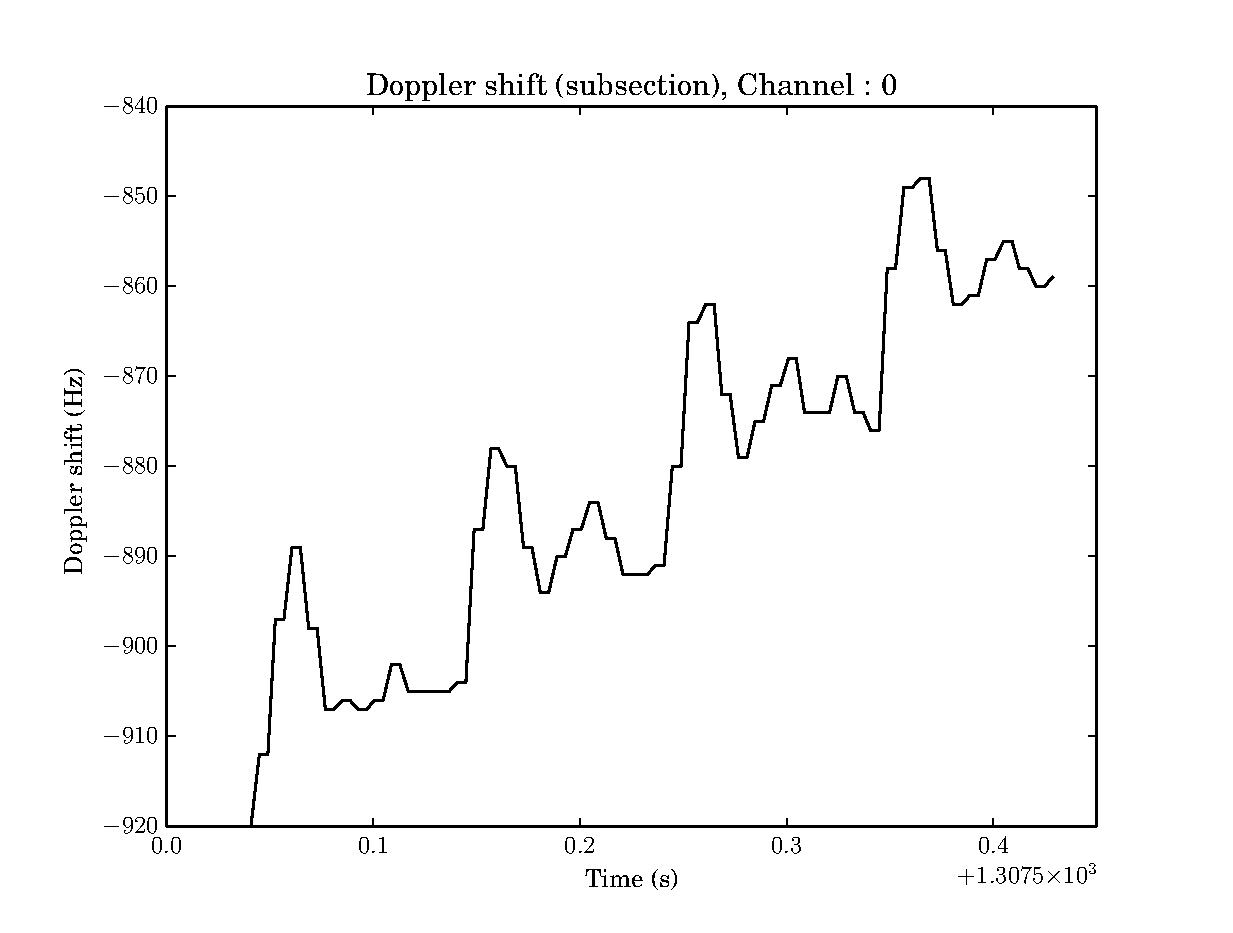
\includegraphics[width=1\textwidth]{SimulatorJitter/DopplerShift0.eps} 
    \caption{The frequency spectrum of the phase errors, note the significant frequency component at 10Hz, and it's harmonics. This component is due to the 10Hz update rate of the simulator.}
    \label{fig:}
\end{figure}


\begin{figure}[!htb] 
    \centering
    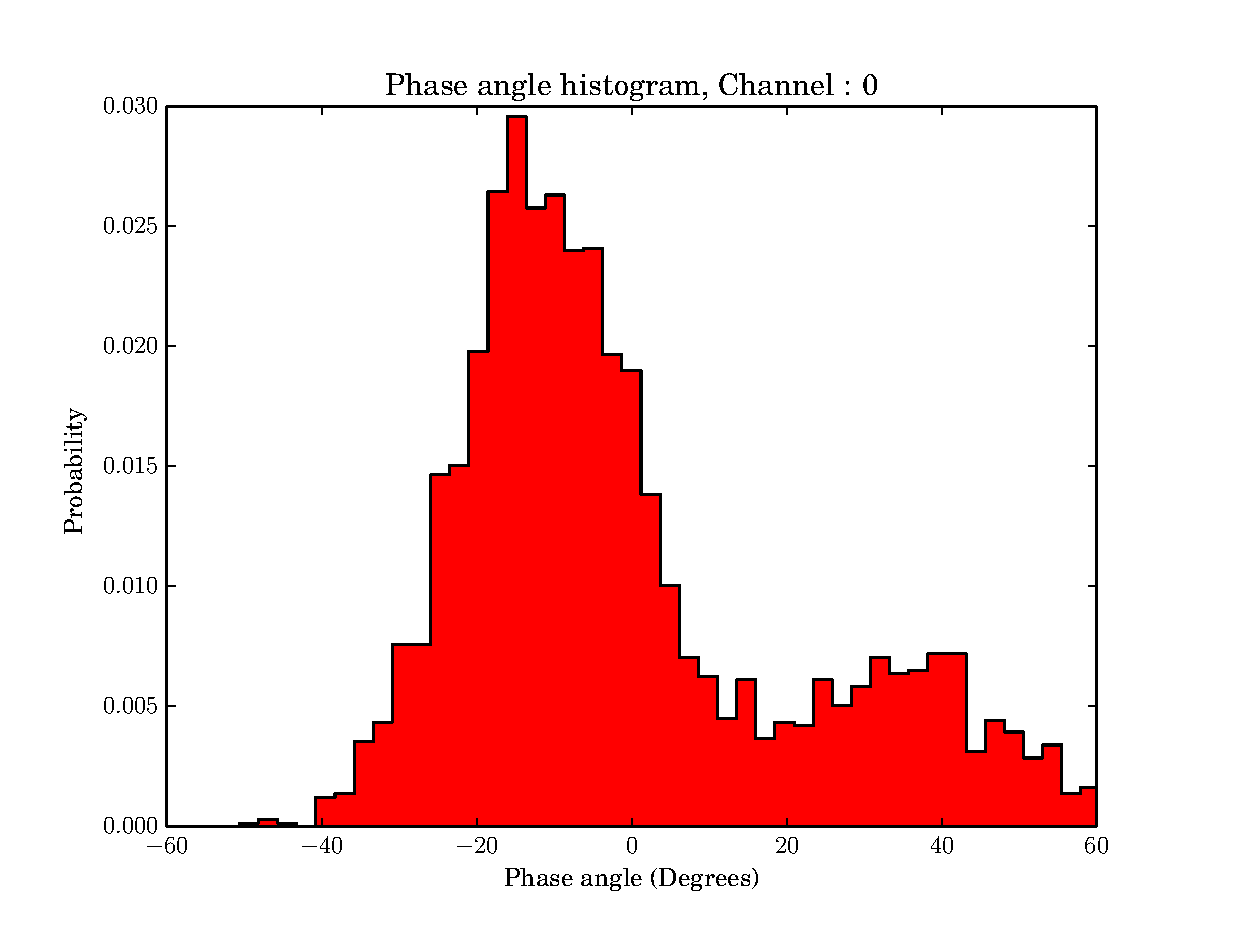
\includegraphics[width=1\textwidth]{SimulatorJitter/PhaseAngleHistogram0.eps} 
    \caption{A histogram of the phase errors. Notice the bimodal nature of the histogram, as opposed to the normal distribution that can be observed in figure \ref{fig:PhaseAngleHistogramStationary}.}
    \label{fig:}
\end{figure}

\begin{figure}[!htb] 
    \centering
    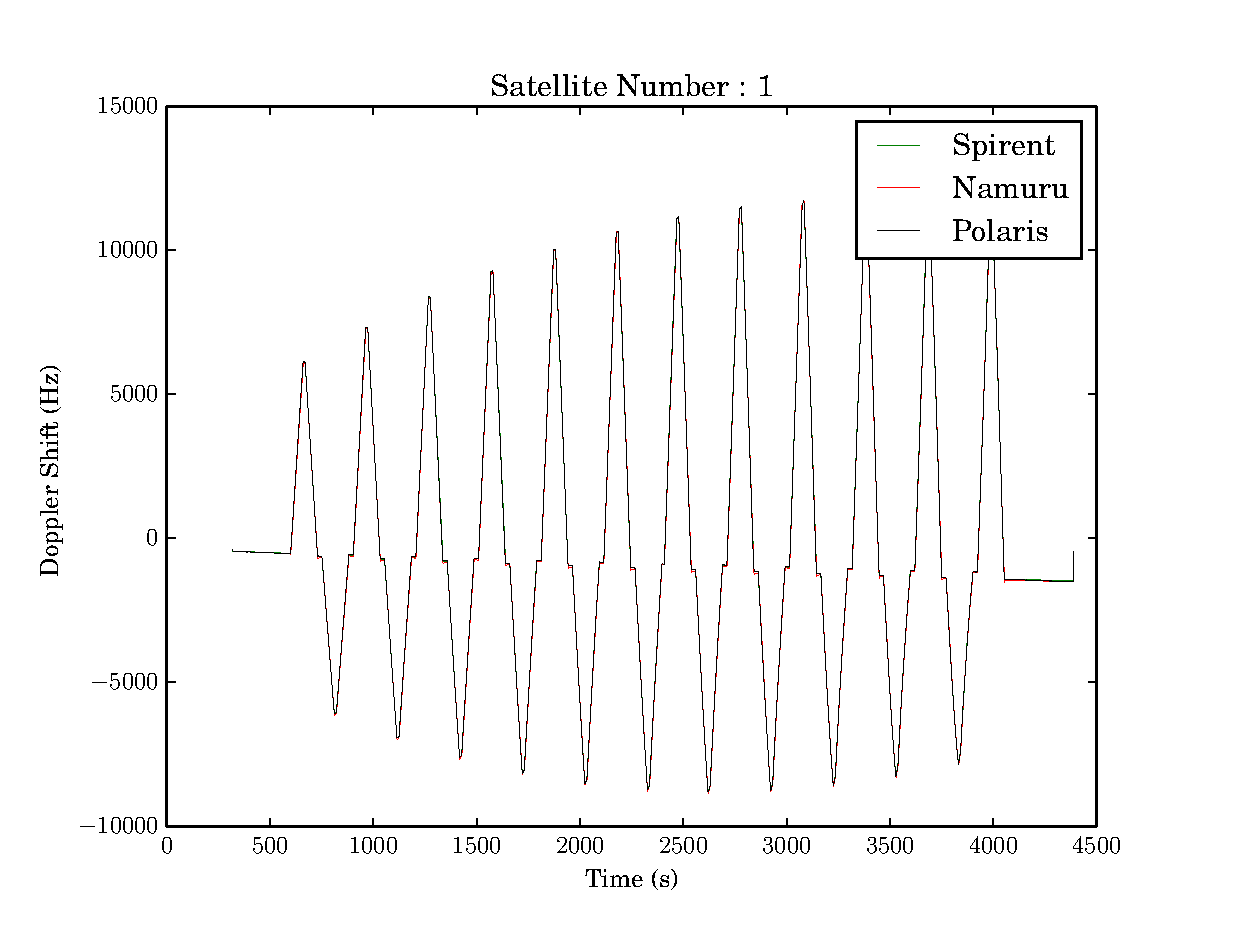
\includegraphics[width=1\textwidth]{SimulatorJitter/1Polaris.eps} 
    \caption{A comparison between the PLL outputs for Spirent, Namuru and Polaris. The Spirent output is the ground truth used in the simulation. The peak \ac{LOS} velocity achieved is approximately 2300m/s.}
    \label{fig:}
\end{figure}



